Tracks can be associated differently to a given calorimeter jet. Compared were tracks that are ghost associated to the ungroomed large-R calorimeter jet and tracks ghost associated to 
the $k_\mathrm{T}$-subjets, which remain after the trimming of the large-R calorimeter jet. 

The distributions showing the number of tracks associated to a calorimeter jet, see the left side of Figure \ref{fig:delta_R}, indicate, that on average around four tracks less are associated to the calorimeter subjets than associated to the whole large-R calorimeter jet. The right side of Figure \ref{fig:delta_R} shows the topological difference between both collections with the angular distance $\Delta R$ between the single tracks, and the axis of the large-R calorimeter jet. Both distributions are aligned in the lower $\Delta R$ region while the histogram representing the tracks associated to the large-R jet shows an enhancement towards larger $\Delta R$. Accordingly, tracks which are not associated to the subjets, but still associated to the ungroomed large-R jet feature an angular separation from the jet axis of more than $0.3$, and are in consequence distributed primarily around the outer regions of the large-R calorimeter jet. Given the required primary vertex association, it is unlikely that these tracks originate from pile-up. Instead, the origin might be found in final- or initial state radiation. 
\begin{figure}
	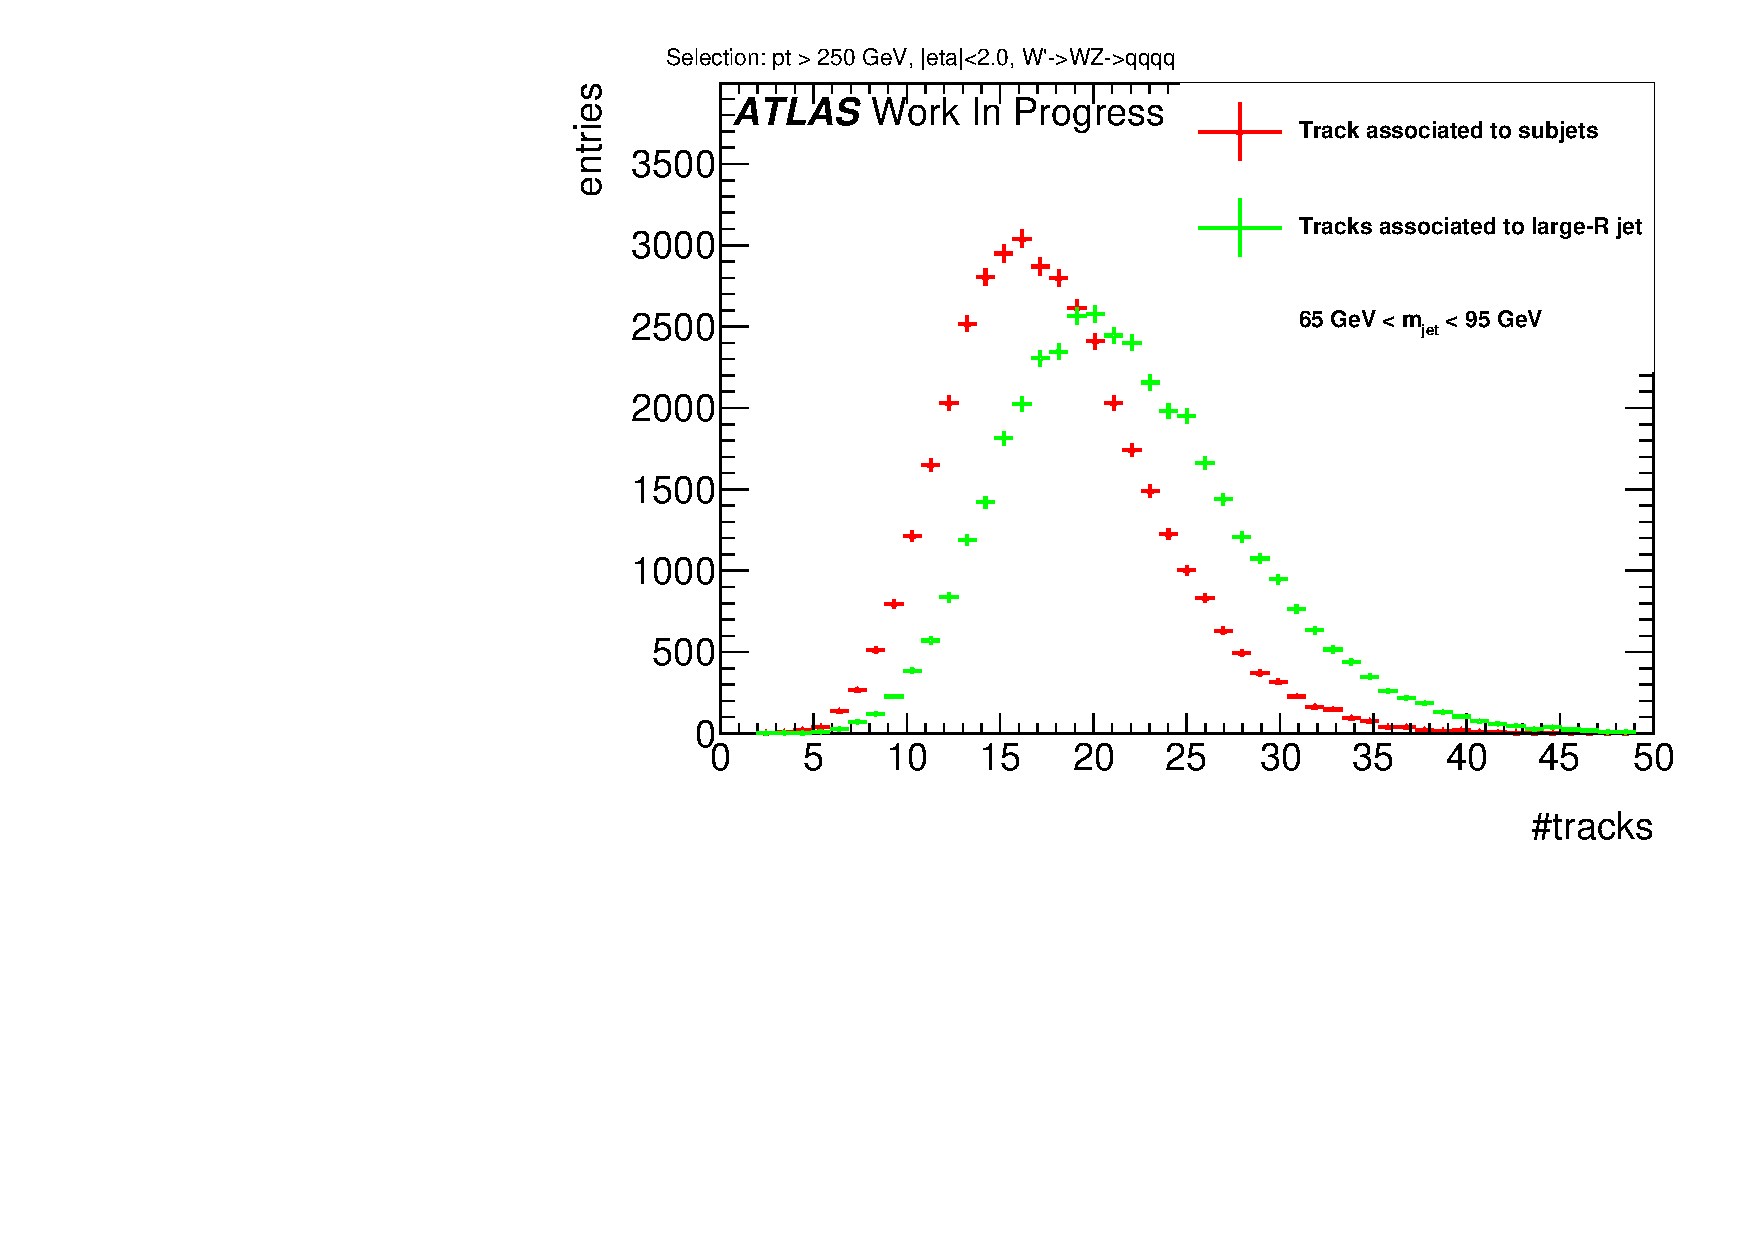
\includegraphics[width=0.5\textwidth]{Main/Results/figures/track_selection/h_customghost_number.pdf} \hspace{1mm}
	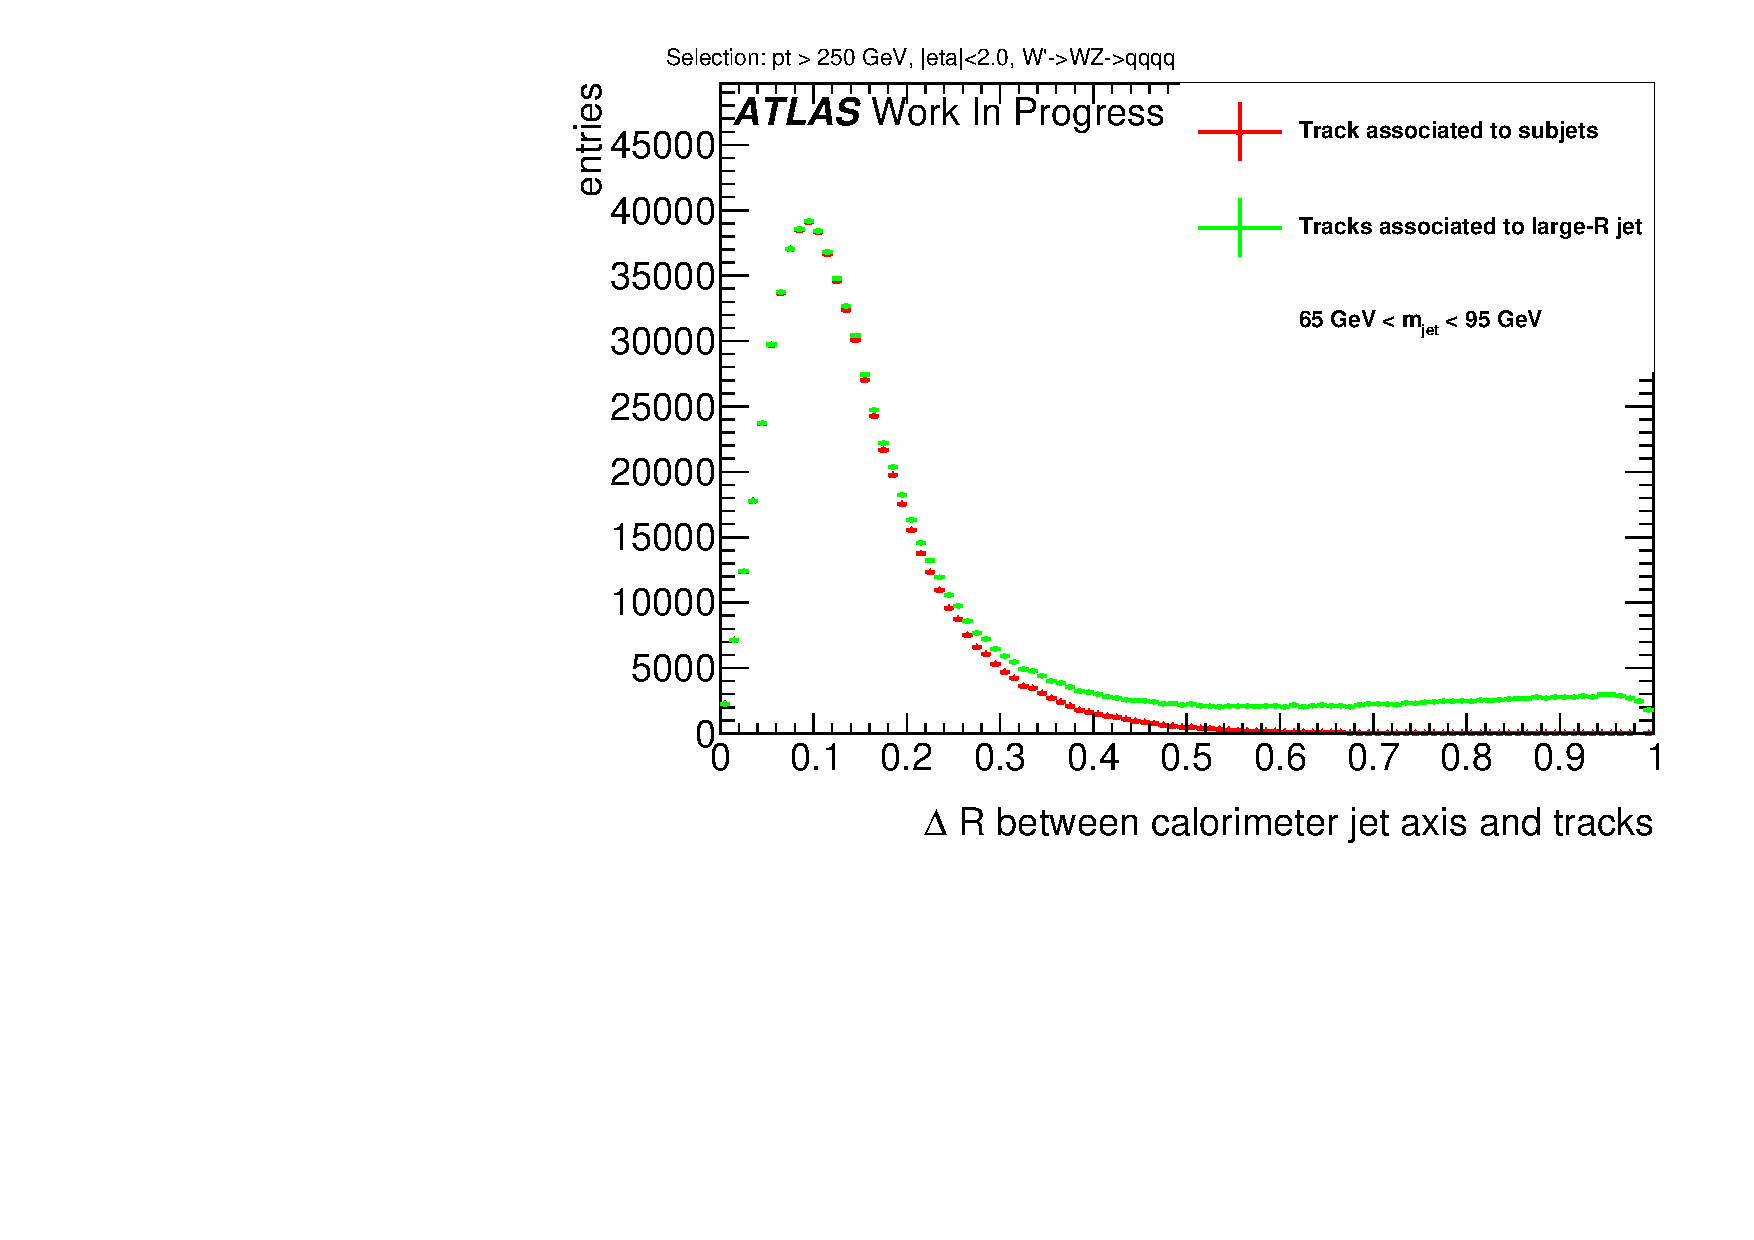
\includegraphics[width=0.5\textwidth]{Main/Results/figures/track_selection/h_customghost_dr.pdf}
\caption{\footnotesize{The number of tracks ghost associated to the large-R jet and to the subjets (left) and angular distance of associated tracks to the large-R calorimeter jet axis (right). Signal events were not reweighted at this step.}}\label{fig:delta_R}
\end{figure}


Figure \ref{fig:selection} shows the signal distributions of the Energy Correlation Double Ratios C2/D2, and the n-Subjettiness ratio $\tau_{21}$, calculated with both selections of tracks for $W$ jets. Especially for C2 and D2, but also for $\tau_{21}$, the signal distributions calculated with tracks associated to the whole calorimeter jet are found to be broader and tending to more background like, higher values compared to the distributions calculated with tracks associated to the subjets. The large $\Delta R$ to the jet axis of the differing tracks push the substructure variables to higher, more background like values. Furthermore, the broader distributions are a result of the variating, large angular distance of the additional tracks. C2 and D2 are more sensitive to tracks with a large $\Delta R$ to the jet axis, since the angular distance between all pairs and triples of tracks is considered For example correlations of tracks on opposite sides of the large-R jet, whereas $\tau_{21}$ uses distances to well defined $k_\mathrm{T}$-WTA axes.
\begin{figure}
	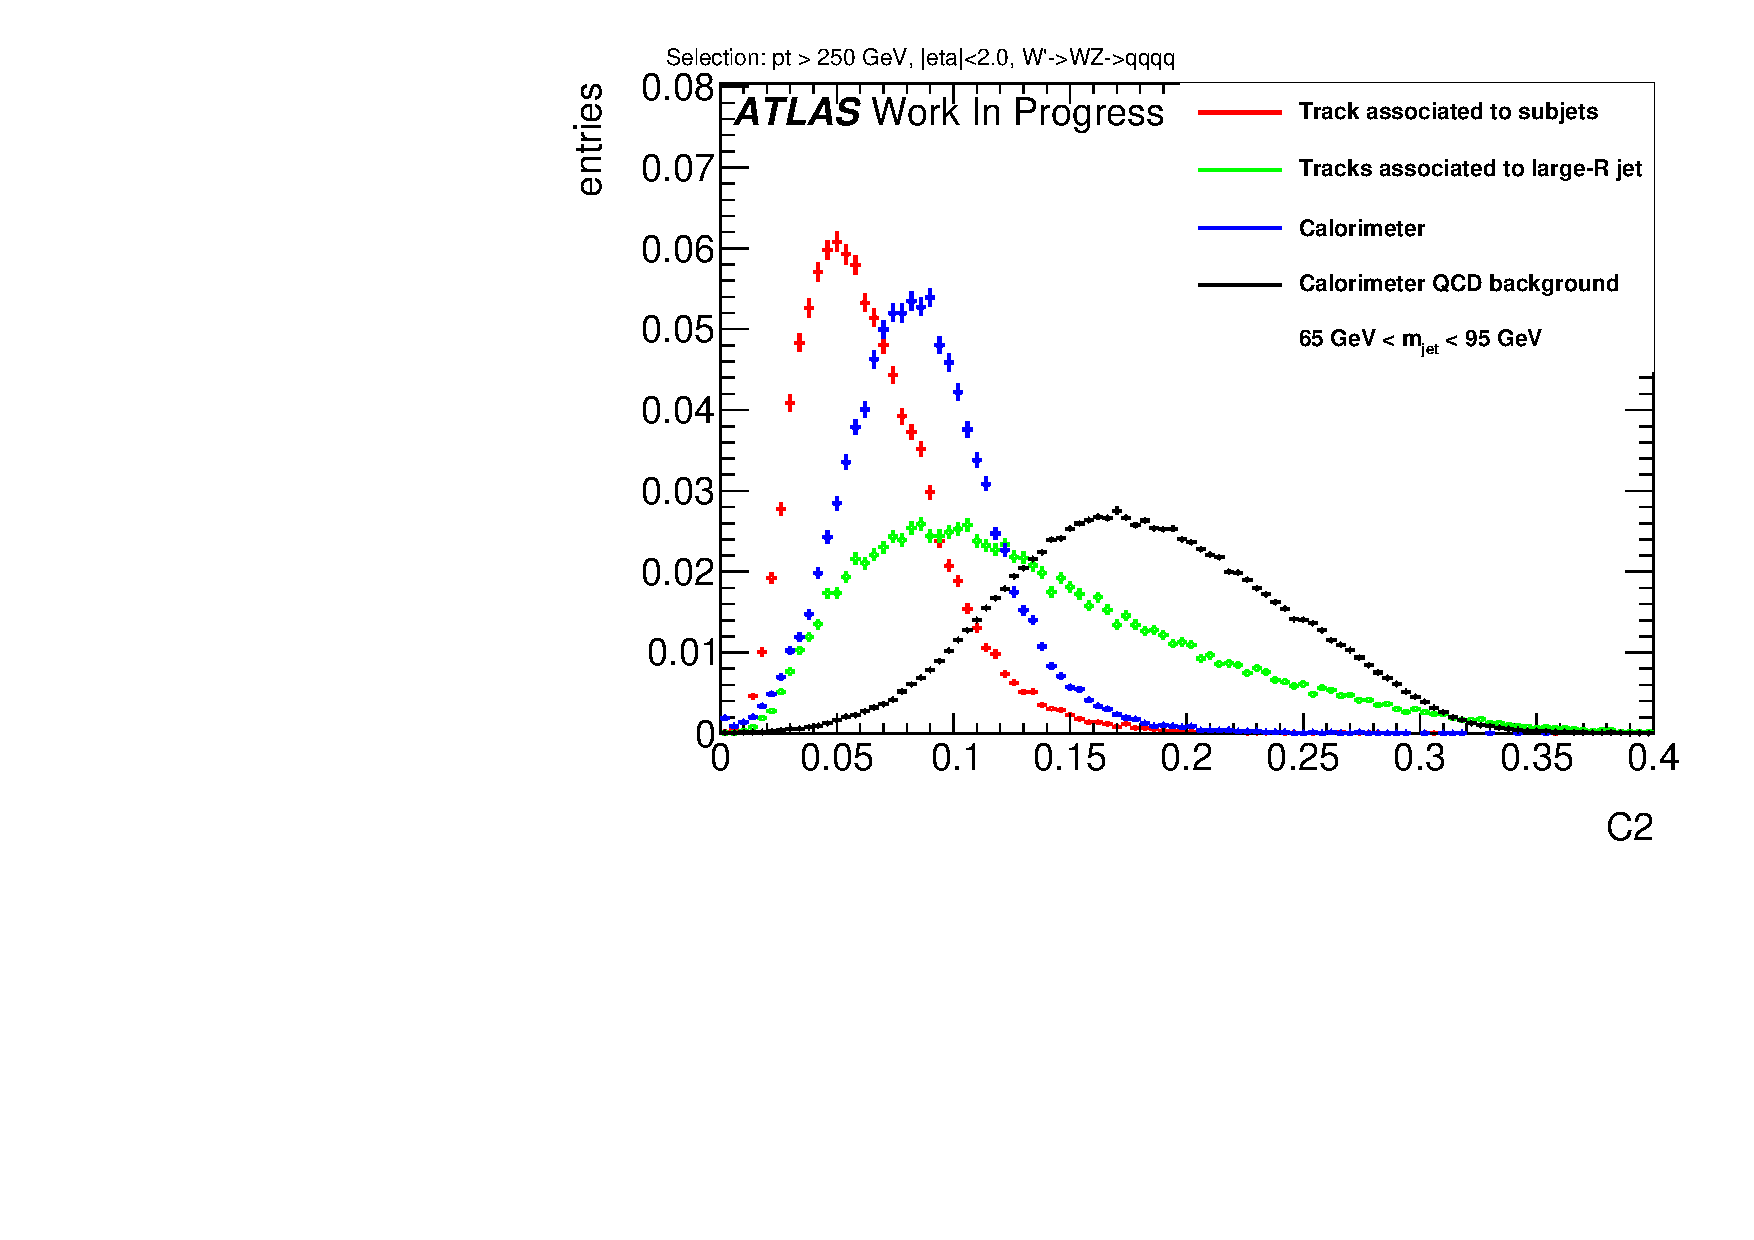
\includegraphics[width=0.5\textwidth]{Main/Results/figures/track_selection/h_ghost_sj_C2.pdf} \hspace{1mm}
	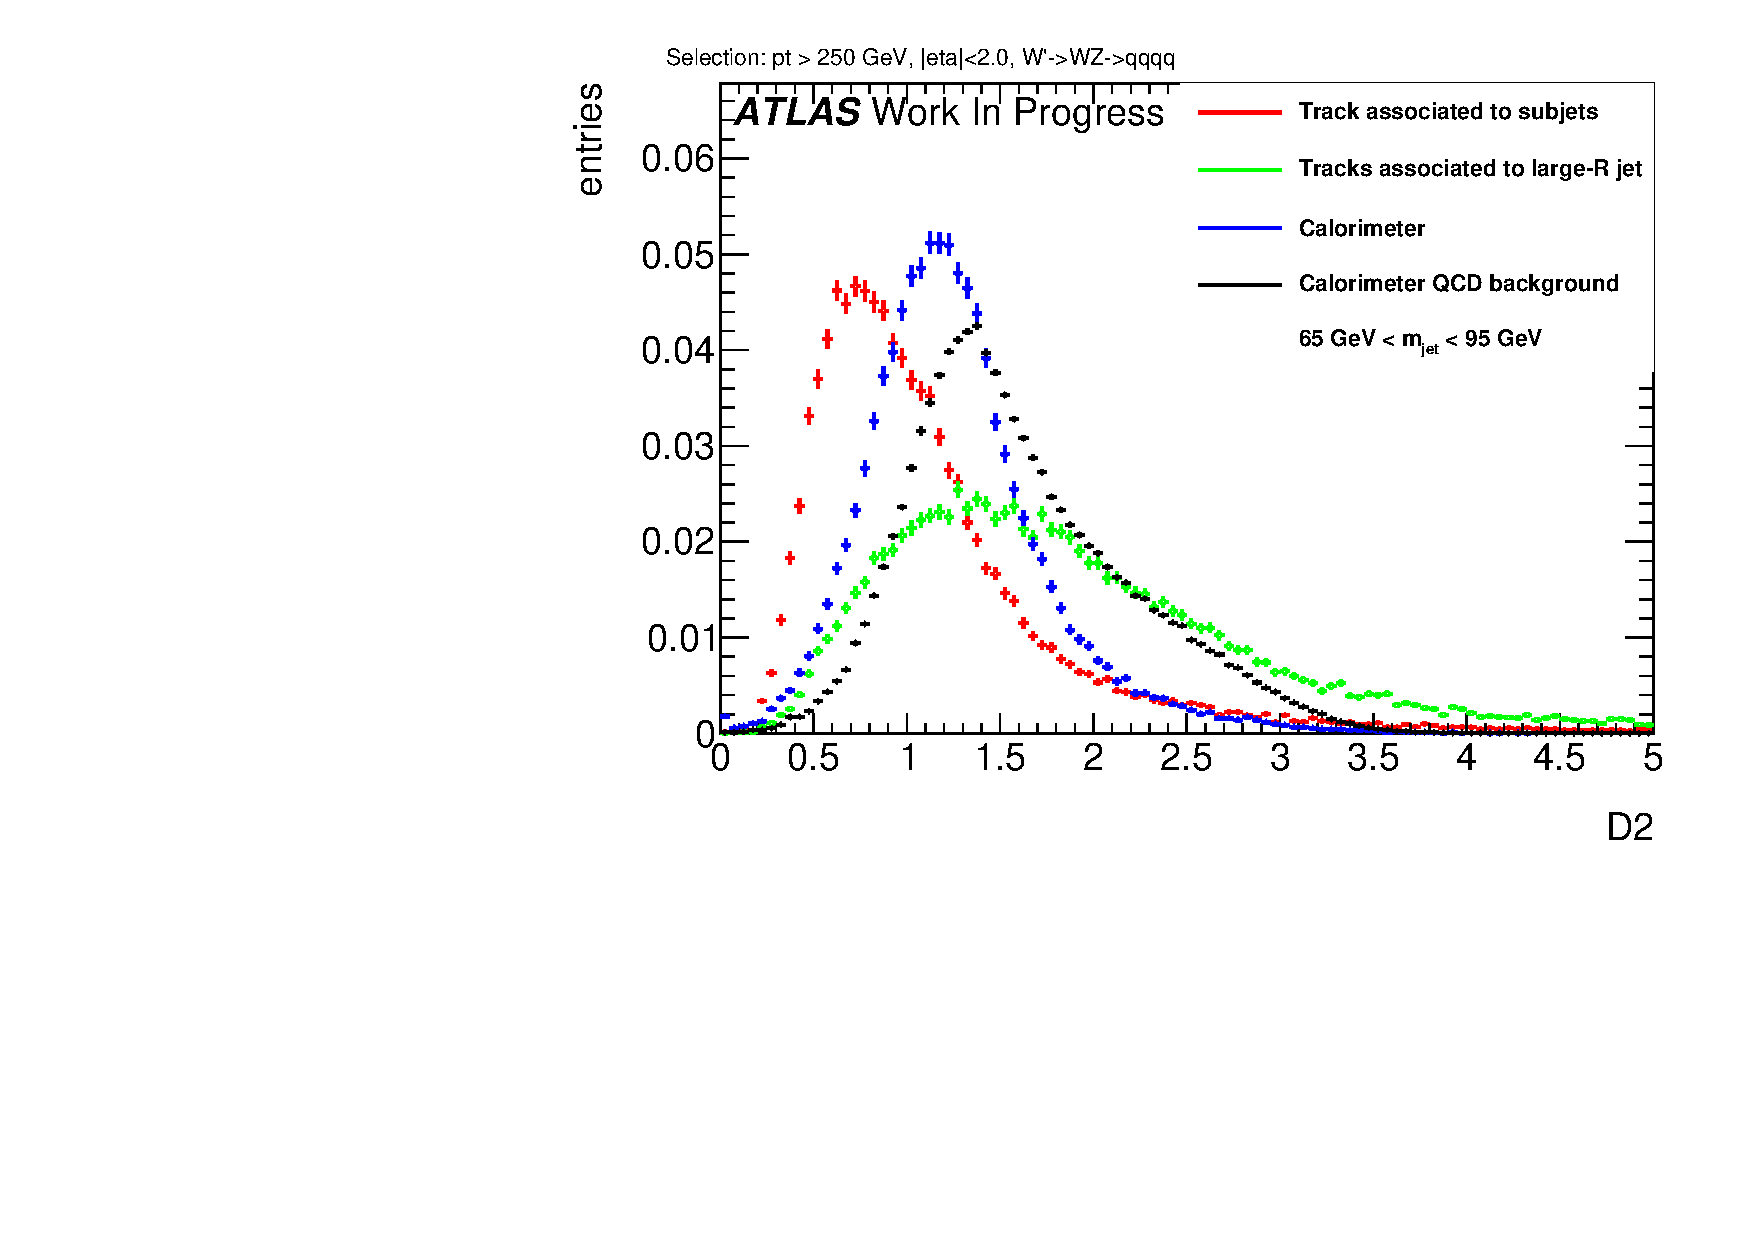
\includegraphics[width=0.5\textwidth]{Main/Results/figures/track_selection/h_ghost_sj_D2.pdf}
	\bigskip
	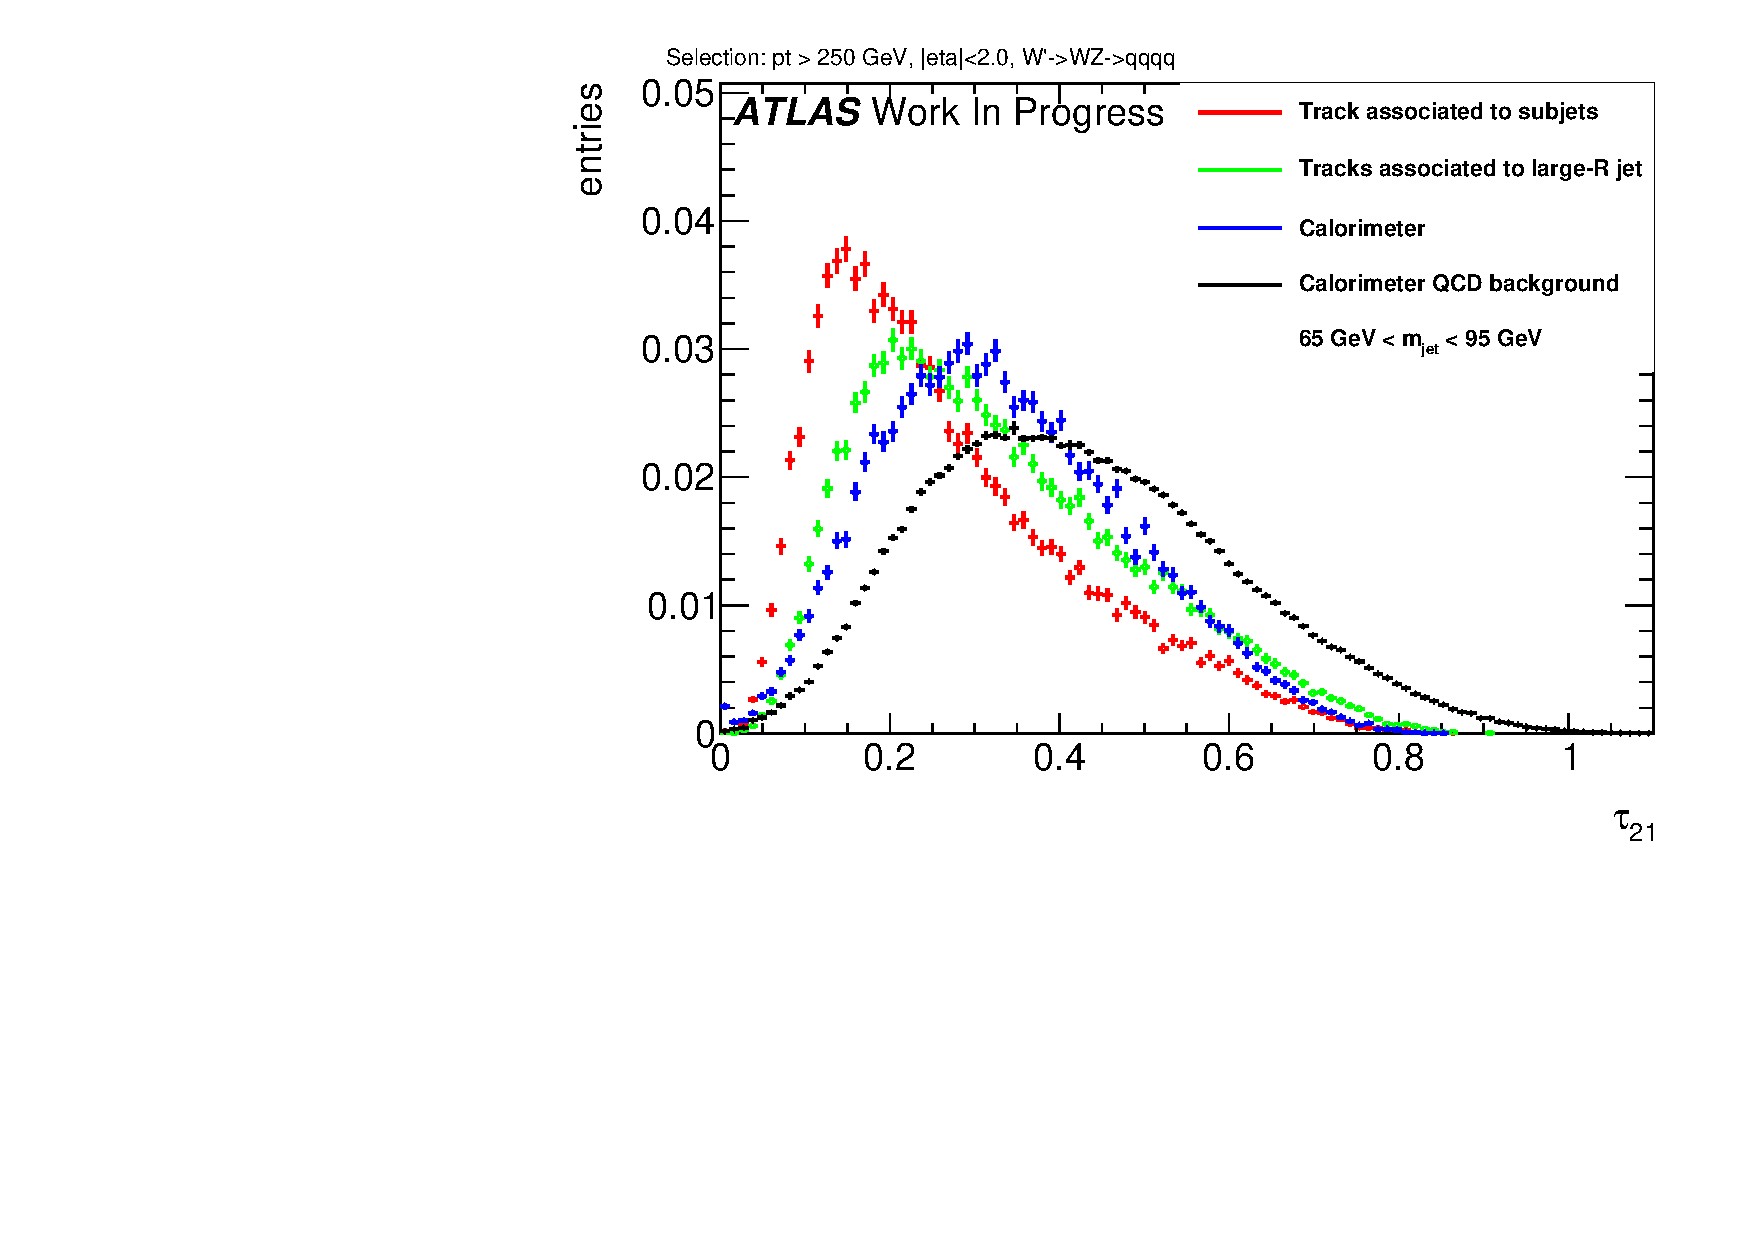
\includegraphics[width=0.5\textwidth]{Main/Results/figures/track_selection/h_ghost_sj_nSub21.pdf}
\caption{\footnotesize{Substructure variables (left) C2, (right) D2 and (below) $\tau_{21}$ calculated with calorimeter clusters as well as tracks associated to subjets and to the large-R jet. Signal events were not reweighted at this step.}}\label{fig:selection}
\end{figure}
For comparison, the signal and background distributions for the variables calculated with calorimeter clusters are shown as well. Through comparing the signal distributions calculated with tracks and clusters, it is possible to anticipate a performance of variables calculated with tracks, that is not worse compared to variables calculated with calorimeter clusters due to the similar width but lower mode of the track distributions.

In contrast, the jet mass variable performs considerably worse with tracks compared to the calorimeter, since the missing information about the fluctuating neutral fraction results in a smaller energy scale and a wider mass distribution. However, the substructure variables studied here are rather energy scale independent and are found to not be as sensitive to the missing fraction.

Starting from this observations, the performance of substructure techniques is compared with the following objects as input:
\begin{itemize}
\item Calorimeter clusters, labeled as 'calo'.
\item Tracks that ghost associated to the calorimeter subjets remaining after trimming, labeled 'tracks'.
\item The same collection of tracks, assisting as defined in Chapter \ref{sec:ta}, labeled 'TAS'.
\end{itemize}